% GRASP method for construction
% Present diferent evaluation functions as well results for each function
\subsection{Construction}
\begin{frame}
  To build a solution, an adjuster is placed at any poiny, after,
  each potential site is evaluated with a greedy function, to obtain a RCL,
  with the $\alpha$ percent of the best solutions.
\end{frame}

\frame{\begin{figure}[h!]\centering{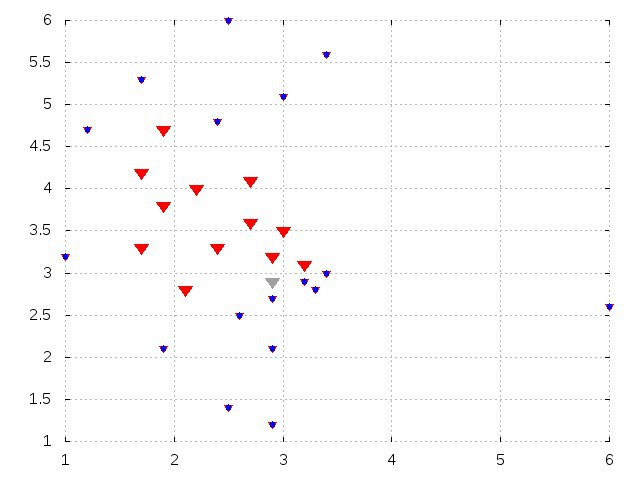
\includegraphics[scale=0.45]{RCL_40_1}\caption{n = m = 30, p = 1, $\alpha$ = 0.4}}\end{figure}}
\frame{\begin{figure}[h!]\centering{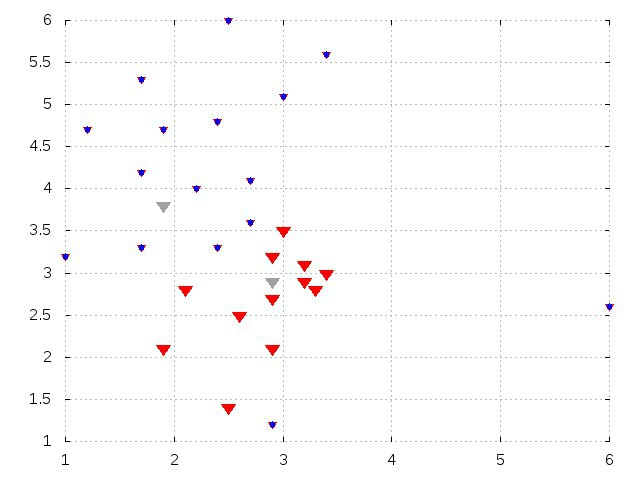
\includegraphics[scale=0.45]{RCL_40_2}\caption{n = m = 30, p = 2, $\alpha$ = 0.4}}\end{figure}}
\frame{\begin{figure}[h!]\centering{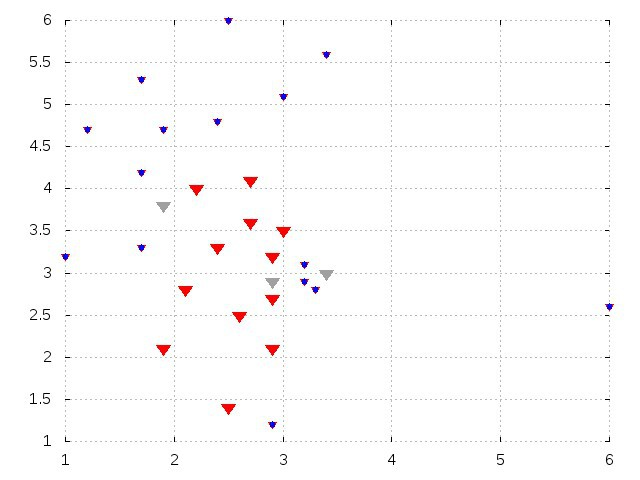
\includegraphics[scale=0.45]{RCL_40_3}\caption{n = m = 30, p = 3, $\alpha$ = 0.4}}\end{figure}}
\frame{\begin{figure}[h!]\centering{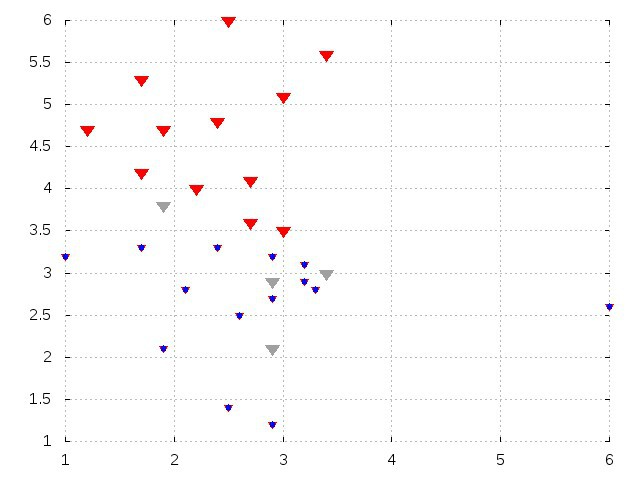
\includegraphics[scale=0.45]{RCL_40_4}\caption{n = m = 30, p = 4, $\alpha$ = 0.4}}\end{figure}}

\subsection{Greedy Functions}
\begin{frame}
  Different greedy functions were evaluated for the construction of solutions using a methodology GRASP.
  \begin{enumerate}
  \item \textbf{p-center} 
    \begin{equation}
      \sum_{i=1}^{p}{\sum_{j|a_{j1}=i}{\tau_{ij}}}
    \end{equation}
  \item \textbf{weighted p-center} 
    \begin{equation}
      \sum_{i=1}^{p}{\sum_{j|a_{j1}=i}{\lambda_{j}\tau_{ij}}}
    \end{equation}
  \item \textbf{K nearest neighbors}
    \begin{equation}
      \sum_{k=1}^K{\sum_{j|a_{jk}=i}{\lambda_{j}\tau_{ij}(1-\rho_i)\prod_{\ell=1}^{k-1}{\rho_{a_{j\ell}}}}}
    \end{equation}
  \end{enumerate}
\end{frame}

\frame{\begin{figure}[h!]\centering{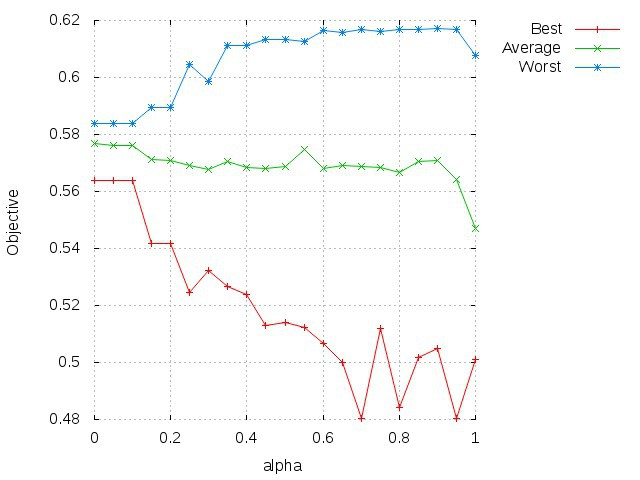
\includegraphics[scale=0.45]{GRASP_30_10_5}\caption{m = 30, n = 10, p = 5}}\end{figure}}
\frame{\begin{figure}[h!]\centering{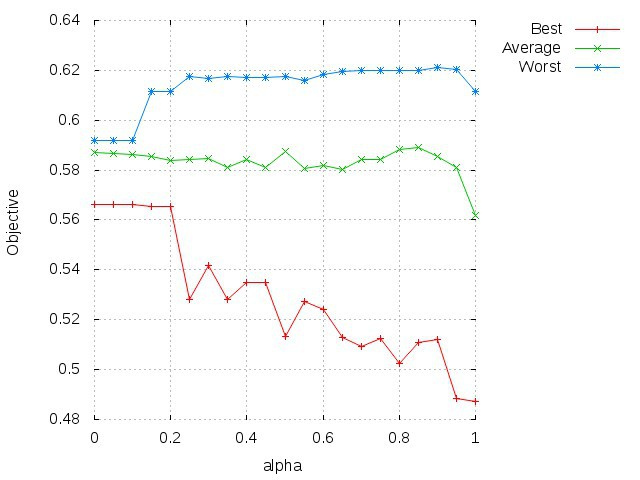
\includegraphics[scale=0.45]{GRASP_30_10_6}\caption{m = 30, n = 10, p = 6}}\end{figure}}
\frame{\begin{figure}[h!]\centering{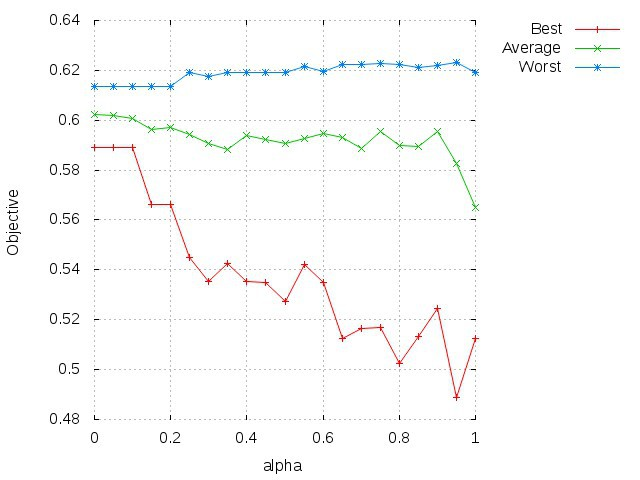
\includegraphics[scale=0.45]{GRASP_30_10_7}\caption{m = 30, n = 10, p = 7}}\end{figure}}
\frame{\begin{figure}[h!]\centering{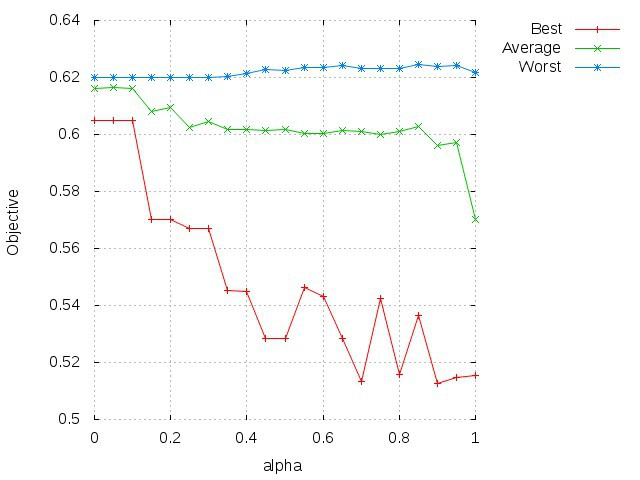
\includegraphics[scale=0.45]{GRASP_30_10_8}\caption{m = 30, n = 10, p = 8}}\end{figure}}


